\chapter{Dynamics of Wheeled Mobile Robots }
\label{c4_Dynamics}
In the field of mobile robotics, extensive research has been carried out. 
Mobile robots can broadly be divided into three categorises, namely wheeled robots, legged robots ~\cite{machado2006overview}, and aerial vehicles ~\cite{valavanis2014handbook}. 
There are few mobile robots which use both wheels and legs for locomotion. For example,  Creadapt  \cite{mouret2015evolutionary} in order to take advantage of both modes of locomotion. 
Among these, the most extensively studied are the  Wheeled Mobile Robots (WMR). 
They have been classified into five generic classes by Champion et. al. \cite{campion1996structural},~\cite{campion2008wheeled}  based on their mobility resulting from the kinematic constrains due to  different wheel types.
 The most common among these are the  3 wheeled differentially driven WMR with one castor wheel.
  Because of its simplicity in modelling, they have been used in most of the  control and motion planing algorithms  \cite{desantis1995modeling}, \cite{koh1999smooth} and \cite{d1995control}. 

In order to develop a model-based control algorithm, it is imperative to have a good dynamic model of the WMR.
 These dynamic models are used in  simulation software,  Software in Loop (SIL) testing and Hardware in Loop (HIL) testing  of the controllers.
 Different methods have  been adopted to derive the dynamic model of WMRs.
  A general dynamical model was derived for three-wheel mobile robots with nonholonomic constraints  by B. d'Andrea-Novel \cite{d1991modelling} using  Lagrange formulation.
    Alternatively, Thanjavur and Rajagopalan \cite{thanjavur1997ease} have used Kane's method,  and  Saha et al. \cite{saha1991dynamics},\cite{saha1989kinematics} used Natural Orthogonal Compliment (NOC) method for the same.  
    
In this chapter we first present the mathamitical model of the mobile robot with two passive wheel at the front. It is then proved using kinematics why a passive wheel with cater offset along the plane of the wheel self orients. This has not been explicitly presented in literature. Using the same set of equations it is proved that zero offset castors must be actuated. 

   
 
%All the papers reviewed use  caster wheel in deriving the dynamic model of a WMR. In this chapter, the modelling is carried out considering the passive wheels in the most general configuration.
% The  castor wheel,  in which the axis of rotation is perpendicular to the line joining the pivot and the axis of rotation, as shown in Figure \ref{fig:std}, is  a special case of the configuration considered here. Whereas in this study they are oriented in  the most general way, as shown in figure Figure \ref{fig:gen}. 
 The concept of the NOC which inherently takes into account the non-holonomic constraint of the wheels has been used. The general methodology of NOC is presented and dynamic model of differential driver robot is presented. 
 The RARS robot has unique  drive configuration, which uses both differential drive and Ackerman mechanism for steering. 
  This system has a redundant configuration and very few literature presents dynamical analysis with slip included in the dynamics. To our knowledge no literature is present, which uses NOC based algorithm for modeling slip in mobile robot dynamics.  This being a matrix based approach, it is convenient for numerical simulations. 
  
   Williams\cite{williams2002dynamic}  and Balakrishna  \cite{balakrishna1995modeling} has presented dynamic equation with slip for omnidirectional robots. 
   While the former has considered both lateral and longitudinal slip assuming the wheel mass to be negligible the later has included the dynamics of  wheels in the dynamics analysis but lateral shift has been considered zero.
    Dynamic model of differential drive robot with wheel slip has been discussed in \cite{tian2009modeling},\cite{sidek2008dynamic}  and \cite{konduri2014effect}.
    Where as the first two has not considered the effect of caster in the dynamic model, \cite{konduri2014effect} has include effect of caster wheels on the dynamic of slip. 
    In this thesis the wheel slip based dynamic model of the redundantly actuated mobile robot has been presented. The effect of steering wheel  miss aliment on the actuator torque has been quantified.

  
  
  
  
  
\section{Modeling using the Natural Orthogonal Compliment (NOC)}
Let us consider a system with $n$ rigid bodies interconnected with different types of joints. 
Let, $f_i$ be the net force acting at the center of mass (CM) of the $i^{th}$  body and $n_i$ is the net moment.
 If $m_i$ is the mass, $I_{ci}$ is the  moment of inertia with respect to the CM, $c_i$ is the position vector of the CM and $\omega_i$ is the angular velocity of the same body, then equations of motion of the $i^{th}$ rigid body are given by Newton-Euler equations as 
\begin{equation}
\label{NE}
f_i=m_i\ddot{c_i} \quad and \quad n_i=I_{ci} \omega_i+\omega_i \times I_{ci} \omega_i
\end{equation}
Let us  define twist ($t$) and wrench($w$) as 
\begin{equation*}
t_i \equiv \begin{pmatrix}
\omega_i\\ \dot{c_i}
\end{pmatrix} \quad
w_i \equiv \begin{pmatrix}
n_i\\f_i
\end{pmatrix}
\end{equation*}
Note that the wrench $w_i$ acting on the $i^{th}$ body can be decomposed into $w^w_i$, called the \textit{working component} and  $w^c_i$, the \textit{non-working component}.
 The working component consists of all the external  moments and forces, which imparts/extracts energy to/from the system, e.g., motor actuating torque.
  The non-working component of the wrench consists of the moments and forces that are used to constrain the motion of the body at the joints.
Then, Newton-Euler equations (\ref{NE}) can be rewritten  in a single matrix equation as 
\begin{equation}
\label{2}
M_i\dot{t_i}+W_iM_it_i=w^w_i+w^c_i \quad \because w_i \equiv w^w_i+w^c_i
\end{equation}
where
\begin{equation}
\label{3}
M_i \equiv \begin{pmatrix}
I_{ci} & 0\\0 & m_i\tilde{1}
\end{pmatrix} ,
\quad W_i\equiv \begin{pmatrix}
\Omega_i &0\\0&0
\end{pmatrix},
\quad
\Omega_i\equiv \omega_i\times \tilde{1}
\end{equation}
in which  $\Omega_i$, is refered as the cross-product matrix of vector $\omega_i$ and $\tilde{1}$ denotes the identity matrix.For details, refer to \cite{angeles2013fundamentals},\cite{saha2010robotics}.If we define 
\[M \equiv diag[M_1,M_2,...M_n], \quad W \equiv diag[W_1,W_2,...W_n], \quad t \equiv [t_1^T,t_2^T, ....t_n^T]^T\] 
and 
\[ w^j \equiv [{w_1^j}^T,{w_2^j}^T, ....{w_n^j}^T]^T, \,j=c,w \]
then the equations of all the $n$ rigid bodies in the system can be collected and written as a single matrix equation 
\begin{equation}
\label{DCE}
M\dot{t}+WMt=w^c+w^w
\end{equation}
 The above equation is referred to as  decoupled equations of motion of the system.



The kinematic constraints, both holonomic and non-holonomic (e.g., pure rolling), between two bodies $i$ and $j$ of a system can be expressed as a linear homogeneous system of algebraic equations \cite{angeles2013fundamentals}, namely 
\begin{equation}
A_it_i+A_jt_j=0
\end{equation}
where $A_i,A_j$ depend on the kinematic parameters.

The constraint equations corresponding to all the joints in the system can be written in terms of the \textit{generalized twist vector} $t$. Furthermore, if $ \dot{\theta} \equiv[\dot{\theta_1},\dot{\theta_2},...\dot\theta_n]^T$ denote the \textit{independent generalized joint rates}. One can then write $t$ in terms of $\dot{\theta}$ as $t=T\dot{\theta}$. 
Using the fact, that $\dot{\theta}$ can take any arbitrary value, we get
\begin{equation}
\label{AT}
At=0 , \quad \Rightarrow  AT\dot{\theta}=0\quad \Rightarrow AT=0
\end{equation}
The Equation \ref{AT} indicates that $T$ is the orthogonal complement of $A$.
 Since this relation arises naturally, hence the name \textit{Natural Orthogonal Complement}.  It can be shown \cite{angeles2013fundamentals} that the non-working wrench $w^c$ lies in the range space of $A^T$.   In view of Equation \ref{AT}, it can be proved that $w^c$ lies in the null space of $T^T$. Therefore,
\begin{equation}
T^Tw^c=0
\end{equation}
To eliminate the non-working  moments and  forces, i.e., $w^c$ from the uncoupled equation of motion (\ref{DCE}), we multiply both sides of the equation  by $T^T$,
\begin{equation}
 T^TM\dot{t}+T^TWMt=T^Tw^W, \quad
 \Rightarrow T^TMT\ddot{\theta}+T^T(M\dot{T}+WMT)\dot{\theta}=T^Tw^w
 \label{eqn:CEM}
\end{equation}
Equation \ref{eqn:CEM} represents the dynamic equation of  interconnected $n$-body system.
 This equation is expressed in terms of the independent generalized joint rates $\dot{\theta}$ and cosponsoring  acceleration $\ddot{\theta}$. Further, using the relations $t=T\dot{\theta}$ and $\dot{t}=\dot{T}\dot{\theta}+T\ddot{\theta}$  in Equation \ref{eqn:CEM}  the final equations of motion can be written as

\begin{equation}
\label{CE}
 \quad I(\theta)\ddot{\theta}+C(\theta,\dot{\theta})\dot{\theta}=\tau
\end{equation}
where
\begin{align*}
I(\theta) &\equiv T^TMT\quad \quad:\text{generalized inertia matrix}\\
C(\theta,\dot{\theta})&\equiv +T^T(M\dot{T}+WMT) \quad :\text{generalized  convective inertia matrix}\\
\tau&\equiv T^Tw \quad \quad :\text{ generalized vector of driving forces }
\end{align*}

Where, 
\begin{equation}
	I(\theta)=\sum_{i=1..n}(T_i^TM_iT_i)
\end{equation}
\begin{equation}
C(\theta,\dot{\theta})=\sum_{i=1..n}(T_i^T M_i\dot{T_i}+T_i W_i M_i T_i)
\end{equation}
\begin{equation}
\tau=\sum_{i=1..n}T_i^T w^w_i
\end{equation}

\begin{figure}
	\begin{minipage}[t]{0.5\textwidth}
	\centering
		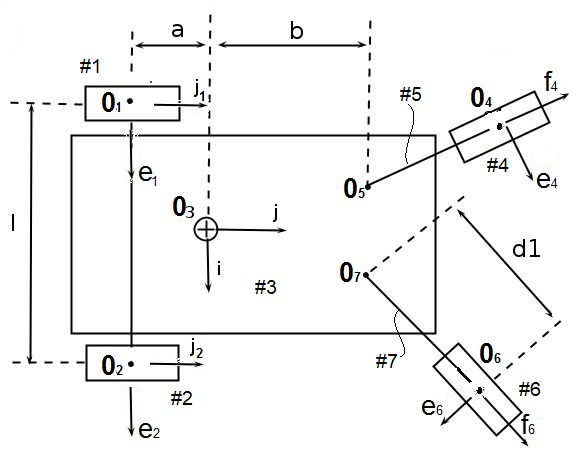
\includegraphics[width=3in]{Chapter4/fig/fig1.jpg} 
		\caption{WMR-Std. castor}\label{fig:std}
	\end{minipage}
	\hfill
	\begin{minipage}[t]{0.5\textwidth}
	\centering
		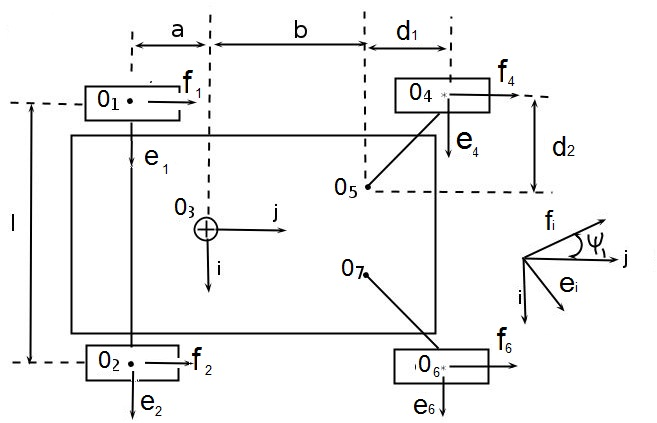
\includegraphics[width=3.5in]{Chapter4/fig/fig2.jpg} 
		\caption{WMR-general}\label{fig:gen}
			\end{minipage}
%\caption{Castor wheel configuration of a WMR}
\end{figure}


\section{Dynamic Equation of WMR}
\label{sec:DynamicNoSlip}
The dynamic equation of a differentially driven 3 wheeled mobile robot based on the  Natural Orthogonal Compliment (NOC) has been presented by Saha~\cite{saha1991dynamics}. The vehicle consisted of 2 driven wheels and one standard caster wheel. In general, for large vehicles, it is necessary to have at least four wheels from the point of stability of the vehicle. Such a vehicle  is shown in Figure \ref{fig:std}. It may be noted that the caster wheels used in this case are the standard caster, where the angle between line $O_4O_5$ and vector $e_4$ is  $90^o$. Which is a special case of the more general configuration of the passive wheels shown in figure \ref{fig:gen}, where angle between line $O_4O_5$ and vector $e_4$ is not $90^o$

 The vehicle considered for analysis in this chapter is shown in Figure \ref{fig:gen}. It consists of two independently driven wheels at the back and two passive wheels at the front. The actuated wheels are labelled as body \#1 and \#2 as indicated in Figure \ref{fig:gen}. The platform is body \#3. The first caster wheel and its bracket is labelled as \#4 and \#5 respectively, with the castor pivoted at $O_5$. Similarly, the second castor is pivoted at $O_7$, and its bracket and wheel are labelled as \#6 an \#7, respectively, all the wheels are assumed to be rolling without slipping.  
\subsection{Kinematic analysis}
In order to proceed with the kinematic analysis of the vehicle in Figure \ref{fig:gen}, we define an orthogonal triad of vectors ${i,j,k}$ at point $O_3$, the control point of the platform, as shown in Figure \ref{fig:gen}. If $\dot{\theta_1}$ and $\dot{\theta_2}$ {( positive when pointing along $i$)} denote the rates of rotation of wheels \#1 and \#2 then the linear velocity of points $O_1$ and $O_2$ under pure rolling condition is given by 
\begin{equation}
\label{velO1}
{\dot{o_i}}=-r\dot{\theta_i}j, \quad \text{r=radius of wheel}
\end{equation}
The angular velocity of the platform $\omega_3$ can be written as 
\begin{equation}
\label{omegaPlat}
{\omega_3}=(r/l)(\dot{\theta_1}-\dot{\theta_2}){k}
\end{equation}
Further, the velocity of point $O_3$ can be written as
${\dot{o_3}=\dot{o_i}+\omega_3 \times (c-o_i)}, \quad i=1,2$, where $o_3 $ and $o_i$  is the position vector of points $O_3$ and $O_i$ respectively, with respect to some  point fixed to the ground. Eliminating $\omega_3$  one gets the following:

\begin{equation}
\label{velPlat}
 \quad \quad \dot{o_3}={(a r/l)(-\dot{\theta_1}+\dot{\theta_2})}i -(r/2)( \dot{\theta_1}+ \dot{\theta_2})j
\end{equation}
Now, the angular velocity of the drive wheel \#1 can be expressed as ${\omega_1}=-\dot{\theta_1}i+\omega_3k$. Using Equation \ref{omegaPlat}, the same can be rewritten as 

\begin{equation}
\label{omegaWheel1}
{\omega_1}=\begin{pmatrix}
-i+(r/l)k & -(r/l)k
\end{pmatrix}
\begin{pmatrix}
\dot{\theta_1}\\\dot{\theta_2}
\end{pmatrix}
\end{equation}
Similarly for the second wheel (\#2) we get
\begin{equation}
\label{omegaWheel2}
{\omega_1}=\begin{pmatrix}
(r/l)k & i-(r/l)k
\end{pmatrix}
\begin{pmatrix}
\dot{\theta_1}\\\dot{\theta_2}
\end{pmatrix}
\end{equation}
Based on  Equations \ref{velO1} and \ref{omegaWheel1}, the twist for wheel \#1 in terms of $\dot{\theta_a}\equiv (\dot{\theta_1},\dot{\theta_2})^T$, can be written as 
\begin{equation}
\label{twist1}
t_1=\begin{pmatrix}
\omega_1\\\dot{o_1}
\end{pmatrix}=
\begin{pmatrix}
i+(r/l)k & -(r/l)k\\- rj & 0
\end{pmatrix}
\begin{pmatrix}
\dot{\theta_1}\\\dot{\theta_2}
\end{pmatrix}
\end{equation}

Similarly, for the other actuated wheel \#2, one gets

\begin{equation}
\label{twist2}
t_2=\begin{pmatrix}
\omega_2\\\dot{o_2}
\end{pmatrix}=
		\begin{pmatrix}
		(r/l)k & i-(r/l)k\\
		  0 & -rj
		\end{pmatrix}
		\begin{pmatrix}
		\dot{\theta_1}\\\dot{\theta_2}
		\end{pmatrix}\\
		\end{equation}

To calculate the twist, $t_3$ of the platform body \#3, Equations \ref{omegaPlat} and \ref{velPlat} are combined to get
\begin{equation}
\label{twist3}
t_3=\begin{pmatrix}
\omega_3\\\dot{o_3}
\end{pmatrix}=
\begin{pmatrix}
\rho\delta & -\rho\delta\\
r(\lambda i+(1/2)j) & r(-\lambda i+(1/2)j)
\end{pmatrix}
\begin{pmatrix}
\dot{\theta_1}\\\dot{\theta_2}
\end{pmatrix}
\end{equation}
where
\[ \delta\equiv d/l, \quad \rho \equiv r/d, \quad \lambda \equiv a/l \]
From the above three equations, one gets 
\[T_1=\begin{pmatrix}i+(r/l)k & -(r/l)k\\ -rj & 0\end{pmatrix}, \quad  
T_2=\begin{pmatrix}	(r/l)k & i-(r/l)k\\  0 & -rj \end{pmatrix}\],
\[T_3=\begin{pmatrix}
	\rho\delta & -\rho\delta\\
	r(\lambda i+(1/2))j & r(-\lambda i+(1/2))j
	\end{pmatrix}\]


In order to calculate the twists of the caster bracket and the caster wheel, it is necessary to express the  un-actuated joint rates, $\dot{\psi_1}$ and $\dot{\phi_1}$, in terms of the actuated joint rate vector $\dot{\theta_a}$. Note here that $\dot{\psi_1}$ denotes the rate of rotation of the bracket body (\#5) about $O_5$ with respect to the platform, and $\dot{\phi_1}$ is the rate of rotation of caster wheel body (\#4) about its axis $e_4$ with respect to the bracket.
\begin{equation*}
\omega_5=\dot{\psi_1}k+\omega_3, \quad \quad \omega_4=\dot{\phi_1} e_4 +\omega_5
\end{equation*}
 The velocity of $O_5$ can be expressed in two independent forms, namely, one in terms of the velocity of $O_3$ and the other one in terms of the velocity of $O_4$, i.e.,
\begin{equation}
\dot{o_5}=\dot{o_4}+\omega_5\times(d_2e_4-d_1f_4), \quad
\dot{o_5}=\dot{o_3}+\omega_3\times(b j - m i)
\end{equation}
On equating the above two equations together, and using the rotation matrix (R) between coordinate system $\{i,j,k\}$ and $\{e_4,f_4,k\}$ given Equation \ref{eqn:RotMatrix}, 

\begin{equation}
\label{eqn:RotMatrix}
R=\begin{pmatrix}
\cos(\psi_1) & -\sin(\psi_1) \\
\sin(\psi_1) & \cos(\psi_1)
\end{pmatrix}
\end{equation}
 the equation in terms $e_4$ and $f_4$, is obtained as

\begin{equation}
(-\dot{\phi_1}r+\dot{\psi_1}d_1)f_3+d_3\dot{\psi_1}e_3=\dot{o_3}
+\omega_3(m\cos\psi_1-b\sin\psi_1-d_1)e_4
\end{equation} 
Taking the dot product of the above equation first with $e_4$ and then with $f_4$, and using Equation \ref{velPlat} for $\dot{o_3}$, one gets
\begin{eqnarray}
\label{unac2act1}
\begin{pmatrix}
d_2&0\\-d_1 &r
\end{pmatrix}
\begin{pmatrix}
\dot{\psi_1}\\ \dot{\phi_1}
\end{pmatrix}
&=&\begin{pmatrix}
(-ar/l)S_{\psi_1}+(r/2)C_{\psi_1}+\delta_1 & 
(ar/l)S_{\psi_1}+(r/2)C_{\psi_1}-\delta_1 \\
(ar/l)C_{\psi_1}+(r/2)S_{\psi_1}+\delta_2 & 
(-ar/l)C_{\psi_1}+(r/2)S_{\psi_1}-\delta_2 
\end{pmatrix}\dot{\theta_a}\nonumber \\
&=&[F_{ij}]\dot{\theta_a}
\end{eqnarray}
where, 
\[ \delta_1=(r/l)(mC_{\psi_1}-bS_{\psi_1}-d2, \quad  \delta_2=(r/l)(mS_{\psi_1}+bC_{\psi_1}+d_1) \]

Similarly, for the other caster wheel one gets,
\begin{align}
\label{unac2act2}
\begin{pmatrix}
d_2&0\\-d_1 &r
\end{pmatrix}
\begin{pmatrix}
\dot{\psi_2}\\ \dot{\phi_2}
\end{pmatrix}
&=\begin{pmatrix}
(-ar/l)S_{\psi_2}+(r/2)C_{\psi_2}-\delta_3 & 
(ar/l)S_{\psi_2}+(r/2)C_{\psi_2}+\delta_3 \\
(ar/l)C_{\psi_2}+(r/2)S_{\psi_2}+\delta_4 & 
(-ar/l)C_{\psi_2}+(r/2)S_{\psi_2}-\delta_4 
\end{pmatrix}\dot{\theta_a}\nonumber \\
&=[G_{ij}]\dot{\theta_a}
\end{align}
where, 
\[ \delta_3=(r/l)(mC_{\psi_2}+bS_{\psi_2}+d2, \quad  \delta_4=(r/l)(mS_{\psi_2}+bC_{\psi_2}+d1 \]




 The angular and the liner velocity of the CM of the caster wheel  \#4, is  written in terms of the co-ordinate frame fixed to the bracket \#5, i.e. $\{e_4,f_4,k\}$, as
\begin{equation}
\label{omegacastor1}
\omega_4=\dot{\phi_1}e_4+(\omega_3+\dot{\psi_1})k, \quad
\dot{o_4}=\dot{\phi_1}e_4
\end{equation}
Using Equations \ref{unac2act1} and \ref{omegaPlat}, the twist $t_4$ can be written as
\begin{equation}
\label{twist4}
t_4=\begin{pmatrix}
\Theta_4\\C_4
\end{pmatrix}\dot{\theta_a}
\end{equation}
Using the definition of $F(i,j)$ in  Equation \ref{unac2act1}, $\Theta_4$ and $C_4$ can be written as 
\[ \Theta_4=[F_{11}e_4+\bar{F_{21}}k \quad F_{12}e_4+\bar{F_{22}}k],\quad 
C_4=r[-F_{11}f_4 \quad -F_{12}f_4]\]
\[\bar{F_{21}}=F_{21}+\rho \delta, \quad \bar{F_{22}}=F_{22}-\rho\delta\]

The angular and the liner velocity of the CM of the caster bracket \#5  expressed in the co-ordinate frame fixed to the bracket is given as
\begin{equation}
\omega_4=\dot{\phi_1}e_3+\dot{\psi_1}k, \quad
\dot{o_4}=\dot{o_4}+\omega_5\times [-df_3]
\end{equation}
Using Equations   \ref{omegaPlat} and \ref{unac2act2}, the twist $t_5$ can next  be expressed as
\begin{equation}
\label{twist5}
t_5=\begin{pmatrix}
\Theta_5\\C_5
\end{pmatrix}\dot{\theta_a}
\end{equation}
where
\[ \Theta_5 \equiv [\bar{F_{21}}k \quad \bar{F_{22}}k],\quad 
C_5\equiv d[(1/2)\bar{F_{21}}e_4-\rho F_{11}f_4 \quad (1/2)\bar{F_{22}}e_4-\rho F_{12}f_4]\]
In a similar manner, the twists $t_6$ and $t_7$  of the other caster wheel and its bracket, respectively can be written as 
\begin{equation}
\label{twist6}
t_6=\begin{pmatrix}
\Theta_6\\C_6
\end{pmatrix}\dot{\theta_a}, \quad t_7=\begin{pmatrix}
\Theta_7\\C_7
\end{pmatrix}\dot{\theta_a}
\end{equation}
Using  $G(i,j)$ defined in  Equation \ref{unac2act2}, $\Theta_6$, $C_6, \Theta_7$ and $C_7$ are given by
\[ \Theta_6 \equiv [G_{11}e_6+\bar{G_{21}}k \quad G_{12}e_6+\bar{G_{22}}k],\quad 
C_6 \equiv r[-G_{11}f_6 \quad -G_{12}f_6]\]
\[ \Theta_7 \equiv [\bar{G_{21}}k \quad \bar{G_{22}}k],\quad 
C_7 \equiv d[(1/2)\bar{G_{21}}e_6-\rho G_{11}f_6 \quad (1/2)\bar{G_{22}}e_6-\rho G_{12}f_6]\]
\[\bar{G_{21}} \equiv G_{21}+\rho \delta, \quad \bar{G_{22}}\equiv G_{22}-\rho\delta\] 
\subsection{Special cases}
Based on the above kinematic equations \ref{unac2act1} and \ref{unac2act2} for the caster wheels two special cases can be recognized one with $d_1=0$ and another ($d_2=0$). The RARS mobile robot designed fall in the second category and hence it requires a steering actuator as discussed below.  
\subsubsection{Standard caster ($d_1=0$) }
The  standard caster wheel configuration can be obtained by setting the value of $d_1=0$. In such condition, the left hand side matrix of  Equations \ref{unac2act1} and \ref{unac2act2} become  a diagonal matrix. Therefore, the first and second row of Equations \ref{unac2act1} and \ref{unac2act2} get divided by $d_2$ and $r$, respectively. The resulting  equations relating the un-actuated joint rate to  actuated joint rates are similar to those reported by \cite{saha1991dynamics},\cite{angeles2013fundamentals}. These passive wheel are self orienting. Hence there is no need for steering motors. 
\subsubsection{Underactuated case ($d_2=0$)}
It can be seen from Equation \ref{unac2act1} that when the \textit{caster offset}, $d_2=0$, the LHS matrix becomes singular. So the unactuated joint rates cannot be determined from $\dot{\theta_a}$. It is therefore essential to have proper caster offset in case we need caster like behaviour from a passive wheel. 

Am alternative solution is to put an extra actuator to control the bracket motion i.e., $\dot\psi_i$. This is the case in Ackerman steering mechanism, where the steering wheel controls the orientation of the front passive wheels of a car
\section{Dynamic equations}
Based on the twists calculated in terms of the independent joint rate vector vector $\dot{\theta_a}$,  the generalized inertia matrix and the matrix of convective inertia term for the coupled equation of motion \ref{CE} can be derived 
\subsubsection{Generalized inertia matrix, $I$}
\label{sec:GIM}
 The equations gives in Section 4.2.1 of the twist of individual body, i.e $t_i=T_i\dot{\theta_a}$ are used to obtain   $t=[t_1^T, t_2^T....t_7^T]^T$ and $t=T\dot\theta$ where  $T=[T_1^T, T_2^T,... T_7^T]^T$. Since the matrix $M$ is block diagonal, the inertia matrix of the full system  denoted by $I$ is given by
\begin{equation}
I=T^TMT=T_1^TM_1T_1+T_2^TM_2T_2+...T_7^TM_7T_7
\end{equation}
Next, the contribution of the rear wheels  to the inertia matrix, i.e., $I_m$ is given by  \[ I_m=\sum_{i=1,2}T_i^TM_iT_i\] or
\begin{equation}
\label{eqn:I_wheel}
I_m=\begin{pmatrix}
I_w+(\rho\delta)^2H++m_wr^2 & -2(\rho\delta)^2H
\\
-2(\rho\delta)^2H &I+(\rho\delta)^2H++m_wr^2
\end{pmatrix} 
\end{equation}
where \[ M_i \equiv\begin{pmatrix}
\tilde{I_w} &0\\0 & m_w\mathbf{1}
\end{pmatrix} , \quad\tilde{I_w}\equiv\begin{pmatrix}
I_w&0&0\\0&H&\\0&0&H
\end{pmatrix}\]. 

Matrix $\tilde{I_w}$ is the $3\times 3$ moment of inertia matrix of the wheel in co-ordinate frame $\{i,j,k\}$, $m_w$ is mass of the motorized wheels    and $\bm{1}$ is the $3\times 3$ identity matrix. If the mass of the platform is $m_p$ and its moment of inertia about vector ${k}$ is $I_p$, then  \cite{angeles2013fundamentals} 
\begin{equation}
\label{eqn:I_platform}
I_3=T^T_3M_3T_3 =I_p(\rho\delta)^2\begin{pmatrix}
1&-1\\-1&1 \end{pmatrix}\\
+m_pr^2\begin{pmatrix}
(1/4)+\gamma^2 & (1/4)-\gamma^2\\(1/4)-\gamma^2 & (1/4)+\gamma^2
\end{pmatrix}
\end{equation}
Similarly, if $m_c$ is the mass of the castor wheel and it is assumed to be a solid disk, then the generalized inertia matrix  can be written as
\begin{align}
I_c=\sum_{i=4,6}T^T_iM_iT_i=(m_cr^2/4)&
\begin{pmatrix}
6F_{11}^2+\bar{F_{21}}^2 & 6F_{11}F_{12}+\bar{F_{21}}\bar{F_{22}}\\
6F_{11}F_{12}+\bar{F_{21}}\bar{F_{22}} & 6F_{12}^2\bar{F_22}
\end{pmatrix}\\ \nonumber
&+\begin{pmatrix}
6G_{11}^2+\bar{G_{21}}^2 & 6G_{11}G_{12}+\bar{G_{21}}\bar{G_{22}}\\
6G_{11}G_{12}+\bar{G_{21}}\bar{G_{22}} & 6G_{12}^2\bar{G_22}
\end{pmatrix}
\end{align}
If the mass of the brackets, i.e., body \#5 and \#7, are small compared to the mass of the caster wheels, then the contributions of $T^T_5M_5T_5$ and $T^T_7M_7T_7$ can be neglected.


\subsubsection{Matrix of convective inertia term $C$}
The matrix of convective inertia terms of Equation \ref{CE} can be broken down into two parts, $T^TM\dot{T}$ and $T^TWMT$.  As can be seen from Equations \ref{twist1}, \ref{twist2} and \ref{twist3},  $T_1,T_2,T_3$ associated with rear wheels and the platform is constant. Therefore \[T^TM\dot{T}=0\]. The generalized inertia matrix  is constant for the rear wheels and the platform, therefore the vector $I_i\omega_i$ is parallel to  $\omega_i, i=1..3$ \[\Rightarrow\omega\times I\omega=0\] \[\Rightarrow T^TWMT =0\]. This shows that contribution of the rear wheels and the platform  to the convective inertia term is zero. Moreover, the mass of the brackets are assumed to be zero, so they also do not contribute to the convective inertia term. Hence
\begin{equation}
\label{Convective}
C=T^TM\dot{T}+T^TWMT=\sum_{i=4,6}T^T_iM_i\dot{T_i}+\sum_{i=4,6}T_i^TW_iM_iT_i
\end{equation}
The expression for the first term is found by using Equations \ref{unac2act1}, \ref{unac2act2}, \ref{twist4} and \ref{twist6}. The terms $\dot{F_{ij}}$ and $\dot{G_{ij}}$ denote the derivatives of the elements of the matrix $F$ and $G$ defined in Equations \ref{unac2act1} and \ref{unac2act2} . To find $\dot{T_4}$ and  $ \dot{T_6}$ we have used the fact $\dot{e_4}=\omega_4 \times e_4 $ and $\dot{e_4}=\omega_6 \times e_6 $. 
\begin{equation}
\label{corr1}
\begin{split}
T^TM\dot{T}=
(m_cr^2/4)& \biggl[ \begin{pmatrix}
6F_{11}\dot{F_{11}}+\bar{F_{21}}\dot{F_{21}} & 6F_{11}\dot{F_{12}}+\bar{F_{21}}\dot{F_{22}}\\
6\dot{F_{11}}F_{12}+\dot{F_{21}}\bar{F_{22}} & 6F_{12}^2\bar{F_{22}}
\end{pmatrix}\\
&+\begin{pmatrix}
6G_{11}\dot{G_{11}}+\bar{G_{21}}\dot{G_{21}} & 6G_{11}\dot{G_{12}}+\bar{G_{21}}\dot{G_{22}}\\
6\dot{G_{11}}G_{12}+\dot{G_{21}}\bar{G_{22}} & 6G_{12}^2\bar{G_{22}}
\end{pmatrix} \biggr]
\end{split}
\end{equation}
\\
The second term of Equation \ref{Convective} i.e, $ \sum_{i=4,6}T_i^TW_iM_iT_i$ evaluates to zero, as shown below. 

Next, consider passive wheel (\#4), using Equation \ref{twist4} and  $W$ defined in the Equation \ref{3} one gets,
\begin{equation}
\label{corr2}
T^T_4W_4M_4T_4=[\Theta_4, C_4]\begin{pmatrix}
\Omega_4 &0\\0&0
\end{pmatrix}
\begin{pmatrix}
I_4&0\\0 &m_4 \mathbf{1}
\end{pmatrix}
\begin{pmatrix}
\Theta_4\\C_4
\end{pmatrix}=\Theta_4\Omega_4I_4\Theta_4
\end{equation}

To evaluate the above equation, we express  all the terms in the coordinate system $\{{e_4,f_4,k}\}$. Moreover, $\omega_4=\Theta_4 \dot{\theta_a}$, using definition of $\Theta_4$ from Equation \ref{twist4} we get \[\omega_4= (F_{11}\dot{\theta_1}+F_{12}\dot{\theta_2})e_4+(F_{21}\dot{\theta_1}+F_{22}\dot{\theta_2})k\] and the cross product matrix of $\omega_4$ as 
\[
 \Omega_4 \equiv \begin{pmatrix}
 0& -(\bar{F_{21}}\dot{\theta_1}+\bar{F_{22}}\dot{\theta_2}) &0\\
 (\bar{F_{21}}\dot{\theta_1}+\bar{F_{22}}\dot{\theta_2}) & 0 & -(F_{11}\dot{\theta_1}+F_{12}\dot{\theta_2}) \\
 0& (F_{11}\dot{\theta_1}+F_{12}\dot{\theta_2}) &0 
 \end{pmatrix}
\]
When the above expressions are substituted in Equation  \ref{corr2}, we get
\begin{equation}
T^T_4W_4M_4T_4=0, \quad \Rightarrow T^TWMT=0
\end{equation} 
Therefore, the matrix of convective inertia term $C$ of Equation \ref{CE}  evaluates to 

\begin{equation}
\label{C_final}
\begin{split}
C=
(m_cr^2/4)& \biggl[ \begin{pmatrix}
6F_{11}\dot{F_{11}}+\bar{F_{21}}\dot{F_{21}} & 6F_{11}\dot{F_{12}}+\bar{F_{21}}\dot{F_{22}}\\
6\dot{F_{11}}F_{12}+\dot{F_{21}}\bar{F_{22}} & 6F_{12}^2\bar{F_{22}}
\end{pmatrix}\\
&+\begin{pmatrix}
6G_{11}\dot{G_{11}}+\bar{G_{21}}\dot{G_{21}} & 6G_{11}\dot{G_{12}}+\bar{G_{21}}\dot{G_{22}}\\
6\dot{G_{11}}G_{12}+\dot{G_{21}}\bar{G_{22}} & 6G_{12}^2\bar{G_{22}}
\end{pmatrix} \biggr]
\end{split}
\end{equation}

All the components of  Equation  \ref{CE}  are now been evaluated, except the $\tau$. These are simply the torques exerted by the actuated wheels. This completes the dynamic model of the WMR with generalized passive wheel configuration.










\subsection{Simulation }
 
The mobile manipulator proposed in Chapter 3  was modelled as a differentially driven robot. The front wheels and steering mechanism were not included in the dynamic model as their masses are too small compared to the  platform. The weight of each wheel is 0.3Kg, the steering mechanism 0.24Kg, whereas the weight of the  platform is 70Kg.

In  simulation the vehicle reference  point $O_3$ is required to trace a circle of radius 5m. As shown in the Figure \ref{fig:CirTrace}. Let, $ \beta$ be the angle between the line joining  point $O_3$ and $O$ with respect to $X-axis$. The function $\beta(t)$ was defined such that the full circle is completed in 60Sec and the velocity and acceleration of the robot is zero at the beginning (t=0) and end of travel (t=60).
\begin{equation}
\label{path}
\beta(t)=\frac{20\pi}{60^3}t^3-\frac{30\pi}{60^4}t^4+\frac{12\pi}{60^5}t^5
%\label{eqn:betafun}
\end{equation}
The initial pose of the vehicle is parallel to the $Y-axis$ i.e. $\beta=0$  as shown  by dotted line in Figure \ref{fig:CirTrace}.

\begin{figure}[H]
	\centering
		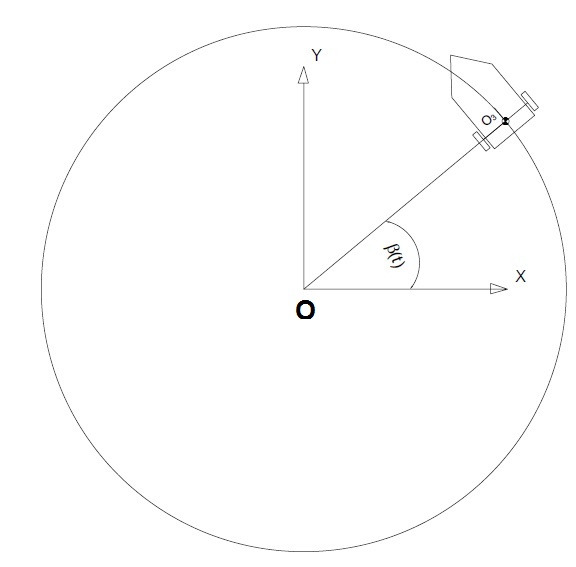
\includegraphics[height=250pt,keepaspectratio]{Chapter4/fig/pathCircle}
		\caption{Path traced by robot}
	\label{fig:CirTrace}
\end{figure}



\subsection{Inverse dynamics}
In order to find the torque required to trace the mobile platform on the circular curve given in Figure \ref{fig:CirTrace}, inverse dynamics was carried out.
Using the model's inverse kinematic,  the wheel velocity and acceleration were determined using pseudo inverse.  % from the equation given below. Where $r$ is radius of the wheel and $\theta_i$ is the wheel roll angle of wheel \#1 and \#2. The platform angular velocity is $\omega$ and the Cartesian velocity of point o3 is given by $\dot{x},\dot{y}$ in body coordinate system %   
The wheel angle, velocity and acceleration were used in the dynamics equation \ref{dnoc}  to calculate the torque required by each motor. The results are plotted in figure \ref{fig:spiral}. 

The equation of  dynamic model  is given in equation \ref{dnoc}, where the actuated joints are  $\theta_a(t)=(\theta_l, \theta_r) $, the rear left and right wheel rotation angles. The dynamic  and kinematic  parameters used in the simulation is listed in table \ref{tb:massproperty}. The rear wheels $(i=1,2)$ and the platform $i=3$, twist $t_i^T=T_i\theta_a$, is given by equations \ref{twist1},\ref{twist2} and \ref{twist3}. The dynamic equation is of the vehicle on slope is given as 
\begin{equation}
\label{dnoc}
\begin{aligned}
T^TMT\ddot{\theta_a}&=-T^T(M\dot{T}+WMT)\dot{\theta_a}+T^T(w^J+w^G)\\
\text{where} \quad &
T=(T_1^T T_2^T T_3^T)^T, \quad M=diag(M_1, M_2, M_3)\\
T^TMT &=I_1+I_2+I_m+I_3= I_m+I_3\\
W&=diag(W_1,W_2,W_3),\quad w^G=g\sin\alpha, \quad \alpha=10^o
\end{aligned}
\end{equation}
where $w^G$, $ w^J$ and $\alpha$ represent the gravitational force acting along the inclined plane,  the external torque applied by a motor and the inclination of the plane to horizontal respectively. The generalized inertia matrix $I_m$ and $I_3$ are given in \ref{eqn:I_wheel} and \ref{eqn:I_platform}.
As stated earlier the convective inertia term is zeros as the inertia matrices are constant. The expression for motor torque  is then given as 
\begin{equation}
T1^Tw_1^j=\tau_1, \quad T_2^Tw_2^j=\tau_2
\end{equation}
\begin{equation}
 T_3^Tw^g=\begin{pmatrix}
\rho\delta k & r(\lambda i+(1/2)j) \\
 -\rho\delta k & r(-\lambda i+(1/2)j)
\end{pmatrix}
\begin{pmatrix}
0\\
-jg\sin\alpha
\end{pmatrix}=\begin{pmatrix}
-\frac{1}{2}rg\sin\alpha\\ -\frac{1}{2}rg\sin\alpha
\end{pmatrix}
\end{equation} 

Figure \ref{fig:spiral} presents the torques required at the wheels of the vehicle while move up a spiral ramp  of slope $10^o$ and radius 5m. 

 \begin{figure}
	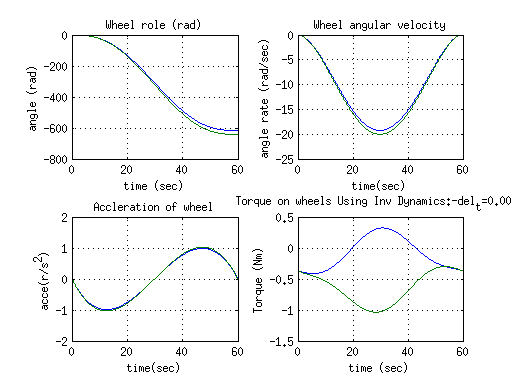
\includegraphics[height=300pt,keepaspectratio]{Chapter4/fig/FD}
	\captionof{figure}{Inverse dynamics of the mobile robot }
	\label{fig:spiral} 
\end{figure} 
%
\begin{table}[!htbp]
	\caption{Dynamic \& kinematic parameters }
	\label{tb:massproperty}
	\centering
	\begin{tabular}{l l l}
		\hline
		\emph{Part Name}  & \emph{ Property} & \emph{Value} \\
		\hline
		Rear Wheels & & \\
		 $m_1,m_2$	& mass				&300g \\ 
		  $I_1,I_2$	& Moment of Inertia	& diag(242, 242, 465)kg $mm^2$\\
		Base Frame& & \\
		 $m_3$ & mass  & 70Kg \\
		 $ I_3$& Moment Of Inertia & $ \begin{pmatrix}
		 1.18& 0.01&-0.05\\ 0.01 & 1.28 & 0.08\\
		 -0.05 & 0.08 & 0.53
		 \end{pmatrix} Kg-m^2$ \\
		   l & length & 400mm\\
		  r & wheel radius (r) & 50mm\\
		 a & see Figure \ref{fig:CirTrace} & 220 mm \\ 
		\hline
		\end{tabular}
\end{table}
\section{Dynamics with Wheel Slip}
\begin{figure}
	\caption{}
	\begin{minipage}[t]{0.5\textwidth}
		\centering
		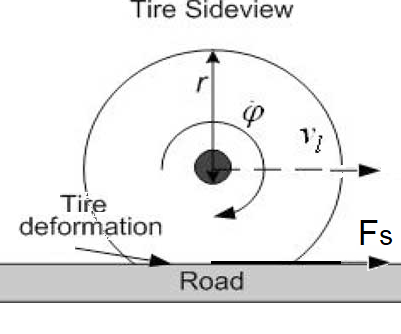
\includegraphics[width=2.5in]{Chapter3/fig/Slip} 
		\caption{Longitudinal slip}\label{fig:slip}
	\end{minipage}
	\hfill
	\begin{minipage}[t]{0.5\textwidth}
		\centering
		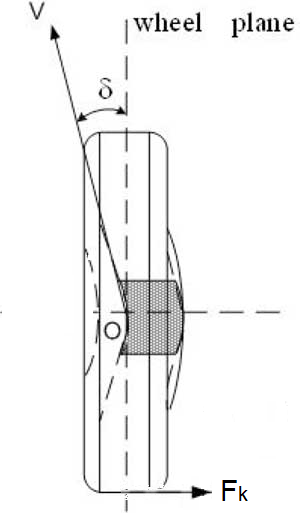
\includegraphics[width=1.5in]{Chapter3/fig/Skid} 
		\caption{Longitudinal Slip or Skid}\label{fig:skid}
	\end{minipage}
\end{figure}
The above derivation of the dynamics of the mobile robot was based on the no slip condition between the ground and the wheel, i.e. pure rolling condition. In case of RARA robot the steering wheels  are passive wheel but power steered, hence it is not assured always that passive wheel will correctly orient itself to assure pure rolling condition of these wheels. Therefore ideal rolling condition removed from the dynamic equation, both the longitudinal slip and lateral slip (also called skid) is introduce.
\subsection{Defining Slip}
\textbf{Longitudinal slip} occurs when the peripheral velocity of the wheel at the point of contact with the ground, $\dot{\phi} \times r$ is different from the linear velocity $v_l$ of the wheel cg as shown in figure \ref{fig:slip}. Where, $\dot{\phi}$ is the angular velocity of wheel and $r$ is the effective radius of the wheel. Under pure rolling assumption  $\dot{\phi} \times r=v_l$. However, this is not the case for a deformed wheel. The wheel slipping can be characterized by
slippage (or Slip ratio) \[\rho = \frac{\dot{\phi} \times r - v_l}{\max(\dot{\phi} \times r,v_l)}\] that has a value range of $ \rho \in [-1, 1]$.  $i = 0$
indicating no wheel slippage whereas $i = 1$ implies a complete slippage, i.e., the wheel is not moving linearly despite its angular rotation. In normal road condition, the wheel's slippage is usually $-1<\rho<1 $. The lateral longitudinal force due to slip is related to the slip ratio $\rho$. One of the well known empirical relation to find $F_s$ is the \textit{ magic formula} \cite{pacejka1992magic} used extensively in automotive industry to modeling Tire forces. 

 \textbf{Lateral slip }also called \textbf{skidding} is experienced when the wheel moves perpendicular to it's plain, this is general encountered during turning. This lateral movement is called skidding. The skidding produces frictional force perpendicular to the wheel plane as shown in figure \ref{fig:skid} by $F_k$. The force $F_k$ is related to the slip angle $\delta$, which is the angle formed between the wheel plane and the velocity vector of the wheel's velocity, when projected on the ground plane.
 The force $F_k$ can again be found using magic formula \cite{pacejka1992magic}. where insted of the slip ratio we use the slip angle as the parameter.
 
 The magic formula \ref{eqn:magic} is reproduced below for completeness. In case of longitudinal slip $Y(x)$ represents longitudinal force $F_s$ and $x$ is the slip ratio $rho$. For computation the lateral frictional force due to skidding $x$ is replaced by the slip angle $\delta$. The constants $D$ represents the peak frictional force. The angle of  tangent at the origin is equal to $BCD$. $C$ controls the shape of the curve, $C=2.4$ for $F_k$ and  $C=1.65$ for $F_s$. $B$ controls the slope at origin. The remaining constant $E$ influences both the curvature of the curve near peak and also the position of$x_m$, where the peak is located.
 
 \begin{equation}\label{eqn:magic}
 Y(x)=D\sin[C \arctan{Bx -E(Bx-\arctan(bx))}]
 \end{equation}
\begin{figure}
	\label{fig:magicformula}
	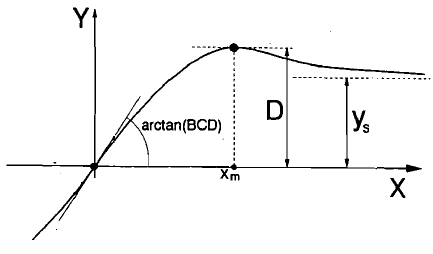
\includegraphics{Chapter3/fig/magicformula}
	\caption{Tipical Curve of Magic Formula \cite{pacejka1992magic}}
\end{figure}

\subsection{Kinematics}
\label{sec:slipKina}
The Figure shows the line digram of the RARS robot. Even though the actual RARS robot uses Ackerman linkage for steering the front wheel, in this we have take the steer angle $\psi_1,\psi_2$ of each wheel independent, this makes the mathematical  model more general. In order to simply things the  link connecting the front wheels to the platform, tie rod etc associated with steering mechanism   are not included in the analysis as there weight is small. The steering axis is assumed to pass through the centre of the front wheel, i.e the offset is zero.  This means $d_1=d_2=0$  for figure \ref{fig:gen}, thus $O_4=O_5$ and $O_6=O_7$. Therefore in Figure \ref{fig:dynslip} we use only $O4$  for wheel \#4 and $O5$ for wheel \#5, to denote both the centre of the wheel and also the steering pivot. DNoc will be used to derive the equations of motion of the RARS with wheel slip taken into account for all the four wheels.


The set of independent variables for this model is given by
\begin{equation}
\label{eqn:theta_slip}
\dot{\theta}_{9x1}=(\dot{\theta_1},\dot{\theta_2}, \dot{y_1},\dot{y_2},\dot{x},\dot{\phi_1},\dot{\phi_2},\dot{\theta_4},\dot{\theta_5})^T
\end{equation}
It may be noted that $\theta_i,\phi_i$  is same as defined earlier in Section \ref{sec:DynamicNoSlip}. $\dot{y_1},\dot{y_2}$ are the linear velocity of centre of the rear wheels i.e. of points point $O_1$ and $O_2$,, in the direction $j$ of the body coordinate system. The lateral slip of the rear wheels are denoted by $x_1$ and $x_2$ as shown in the Figure \ref{fig:dynslip}. Due to rigidity constrains of the rear wheels
\[\dot{x_1}=\dot{x_2}=\dot{x}\] 
The velocity of point $o_1$ and $ o_2$ in the world coordinate ${X,Y,z}$ is given by 
\begin{equation}
\label{eqn:slip_do1}
\dot{o_1}=\dot{x}i +\dot{y_1}j, \quad \quad  \dot{o_2}=\dot{x}i +\dot{y_2}j
\end{equation}
Equating the velocity of point $O_3$ expressed in terms of $o_1$ and $o_2$, We get
\begin{equation}
\label{eqn:slip_do3_rel}
\dot{o_3}=\dot{o_1}+\omega_3\times o_1o_3=\dot{o_2}+\omega_3\times o_2o_3
\end{equation}
Where, $\omega_3$ is the angular velocity of platform, body \#3.
\begin{equation}
	\label{eqn:slip_domega3}
	\omega_3=\frac{\dot{y_2}-\dot{y_1}}{l} k =\bar{\omega_3}k
\end{equation}
using Equations \ref{eqn:slip_do3} and \ref{eqn:slip_domega3} , we get
\begin{equation}
\label{eqn:slip_do3}
\dot{o_3}=(\dot{x}+\frac{a\dot{y_1}}{L}-\frac{a \dot{y_2}}{L})i+(\frac{\dot{y_1}}{2}+\frac{\dot{y_2}}{2})j
\end{equation}
We can write twist $t_3$ for body \#3 as
\begin{equation}
\label{eqn:slip_t3}
t_3=
\begin{pmatrix}
\omega_3\\
\dot{o_3}
\end{pmatrix}=T_3 \dot{\theta}, \quad \text{Where,} \quad 
T_3=
\begin{pmatrix}
0 & 0& -k/l & k/l & 0 &0 & 0 &0 &0\\
0 & 0& ai/l+ j/2& -ai/l+j/2 & 0 &0 & 0 &0 &0\\ 
\end{pmatrix}
\end{equation}
or in expanded form
\begin{equation}
\label{eqn:slip_T3}
T_3=\left(
\begin{array}{ccccccccc}
0 & 0 & 0 & 0 & 0 & 0 & 0 & 0 & 0 \\
0 & 0 & 0 & 0 & 0 & 0 & 0 & 0 & 0 \\
0 & 0 & -\frac{1}{L} & \frac{1}{L} & 0 & 0 & 0 & 0 & 0 \\
0 & 0 & \frac{a}{L} & -\frac{a}{L} & 1 & 0 & 0 & 0 & 0 \\
0 & 0 & \frac{1}{2} & \frac{1}{2} & 0 & 0 & 0 & 0 & 0 \\
0 & 0 & 0 & 0 & 0 & 0 & 0 & 0 & 0
\end{array}
\right)
\end{equation}
Using the fact \[\frac{d i}{dt}=\bar{\omega_3}k\times i =\bar{\omega_3}j, \quad  \frac{d j}{dt}=\bar{\omega_3}k\times j =-\bar{\omega_3}i, \frac{d k}{dt}=\bar{\omega_3}k\times k =0 \] 
\begin{equation}
\label{eqn:slip_dT3}
\dot{T_3}=\begin{pmatrix}
0 & 0& 0 & 0 & 0 &0 & 0 &0 &0\\
0 & 0&-\frac{ \bar{\omega_3}}{2}i +\frac{a \bar{\omega_3}}{l}j& -\frac{ \bar{\omega_3}}{2}i -\frac{a \bar{\omega_3}}{l}j & 0 &0 & 0 &0 &0\\ 
\end{pmatrix}
\end{equation}

The angular velocities $\omega_1$ and $\omega_2$ of wheels \#1 and \#2 is given as
\begin{equation}
\label{eqn:slip_omega1and2}
\omega_1=\dot{\theta_1}i+\omega_3, \quad \omega_2=\dot{\theta_2}i+\omega_3
\end{equation}
using Equations\ref{eqn:slip_do1} and \ref{eqn:slip_omega1and2} for wheel \#1 we get the twist matrix as 
\begin{equation}
\label{eqn:slip_t1}
t_1=
\begin{pmatrix}
\omega_1\\
\dot{o_1}
\end{pmatrix}=T_1 \dot{\theta}
\end{equation} 
\begin{equation}
\label{eqn:slip_T1}
T_1=
\begin{pmatrix}
i & 0& -k/l & k/l & 0 &0 & 0 &0 &0\\
0 & 0& j& 0 & i &0 & 0 &0 &0\\ 
\end{pmatrix}=
\left(
\begin{array}{ccccccccc}
1 & 0 & 0 & 0 & 0 & 0 & 0 & 0 & 0 \\
0 & 0 & 0 & 0 & 0 & 0 & 0 & 0 & 0 \\
0 & 0 & -\frac{1}{L} & \frac{1}{L} & 0 & 0 & 0 & 0 & 0 \\
0 & 0 & 0 & 0 & 1 & 0 & 0 & 0 & 0 \\
0 & 0 & 1 & 0 & 0 & 0 & 0 & 0 & 0 \\
0 & 0 & 0 & 0 & 0 & 0 & 0 & 0 & 0
\end{array}
\right)
\end{equation}

and 
\begin{equation}
\label{eqn:slip_dT1}
\dot{T_1}=\begin{pmatrix}
\bar{\omega_3}j & 0& 0& 0 & 0 &0 & 0 &0 &0\\
0 & 0& -\bar{\omega_3}i& 0 & \bar{\omega_3}j &0 & 0 &0 &0\\ 
\end{pmatrix}
\end{equation}

Using Equations\ref{eqn:slip_do1} and \ref{eqn:slip_omega1and2} for wheel \#2 we get the twist matrix $t_2$  as 
\begin{equation}
\label{eqn:slip_t2}
t_2=
\begin{pmatrix}
\omega_2\\
\dot{o_2}
\end{pmatrix}=T_2 \dot{\theta}
\end{equation} 
\begin{equation}
\label{eqn:slip_T2}
T_2=
\begin{pmatrix}
0 & i& -k/l & k/l & 0 &0 & 0 &0 &0\\
0 & 0& 0& j &i &0 & 0 &0 &0\\ 
\end{pmatrix}=
\left(
\begin{array}{ccccccccc}
0 & 1 & 0 & 0 & 0 & 0 & 0 & 0 & 0 \\
0 & 0 & 0 & 0 & 0 & 0 & 0 & 0 & 0 \\
0 & 0 & -\frac{1}{L} & \frac{1}{L} & 0 & 0 & 0 & 0 & 0 \\
0 & 0 & 0 & 0 & 1 & 0 & 0 & 0 & 0 \\
0 & 0 & 0 & 1 & 0 & 0 & 0 & 0 & 0 \\
0 & 0 & 0 & 0 & 0 & 0 & 0 & 0 & 0
\end{array}
\right)
\end{equation}

and 
\begin{equation}
\label{eqn:slip_dT2}
\dot{T_2}=\begin{pmatrix}
0 & \bar{\omega_3}j & 0& 0 & 0 &0 & 0 &0 &0\\
0 & 0& 0& -\bar{\omega_3}i & \bar{\omega_3}j &0 & 0 &0 &0\\ 
\end{pmatrix}
\end{equation}


Next  the angular velocity of the steered wheel i.e body \#4 relative to the absolute frame is given as 
\[\omega_4=\dot{\theta_4}e_4+ \dot{\psi_1} k +\omega_3\]
The transformation matrix between the Frame $\{e_4,f_4\}$ is given by the rotation matrix $R_4$. From Figure $R_4$ can be written as 
\begin{equation}
\label{eqn:slipR4}
R_4=\begin{pmatrix}
\cos \psi_1 & - \sin \psi_1\\
\sin \psi_1 & \cos\psi_1
\end{pmatrix}
\end{equation}
Then, $e_4= \cos\psi_1 i +\sin \psi_1 j$  and $\omega_4$ can be written as 
\[ \omega_4= \dot{\theta_4}( \cos\psi_1 i +\sin \psi_1 j)+ \dot{\phi_1} k +\omega_3 \]
Linear velocity of point $o_4$ is given as 
\[ \dot{o_4}=\dot{o_3}+\omega_3 \times (-\frac{c}{2}i+bj) \]
or
\begin{equation}
\label{eqn:slip_t4}
t_4=
\begin{pmatrix}
\omega_4\\
\dot{o_4}
\end{pmatrix}=T_4 \dot{\theta}
\end{equation}
where 
\begin{equation}
\label{eqn:slip_T4}
T_4=\left(
\begin{array}{ccccccccc}
0 & 0 & 0 & 0 & 0 & 0 & 0 & \text{Cos}[\text{$\psi $1}] & 0 \\
0 & 0 & 0 & 0 & 0 & 0 & 0 & \text{Sin}[\text{$\psi $1}] & 0 \\
0 & 0 & -\frac{1}{L} & \frac{1}{L} & 0 & 1 & 0 & 0 & 0 \\
0 & 0 & \lambda_1 & -\lambda_1 & 1 & 0 & 0 & 0 & 0 \\
0 & 0 &\lambda_3 & \lambda_2 & 0 & 0 & 0 & 0 & 0 \\
0 & 0 & 0 & 0 & 0 & 0 & 0 & 0 & 0
\end{array}
\right)
\end{equation}
\begin{equation}
\label{eqn{:slip_dT4}}
\dot{T_4}=\begin{pmatrix}
0 & 0 & 0 & 0 & 0 & 0 & 0 & \lambda_4 & 0\\
0 & 0 & \lambda_7 & \lambda_6 & \bar{\omega_3}j & 0 & 0 & 0 & 0
\end{pmatrix}
\end{equation}

 \[\lambda_1=\frac{a+b}{l}, \quad \lambda_2=\frac{l-c}{2l}, \quad \lambda_3=\frac{l+c}{2l} \]
  \[\lambda_4=(\bar{\omega_3}+\dot{\psi_1}) (\cos\psi_1 j-\sin \psi_1 i) \]
  \[\lambda_6=-\bar{\omega_3}(\lambda_1 j+\lambda_2 i), \quad \lambda_7=\bar{\omega_3}(\lambda_1 j-\lambda_3 i)\]
Next, for wheel \#5 
\[\omega_5 = \dot{\theta_5} (R_5.e_5) + \dot{\psi_2} k + \omega_3 =
  \left(
\begin{array}{c}
\dot{\theta }_5 \cos \psi_2 \\
\dot{\theta_5} \sin \psi_2 \\
\dot{\psi_2}+\frac{-\dot{y_1}+\dot{y_2}}{L}
\end{array}
\right) \]
the linear velocity of point $o_5$ is given as 
\[ \dot{o_5}=\dot{o_3}+\omega_3 \times o_3o_5\]
where, \begin{equation}
\label{eqn:slipR5}
R_5=\begin{pmatrix}
\cos \psi_2 & - \sin \psi_2\\
\sin \psi_2 & \cos\psi_2
\end{pmatrix}
\end{equation}
Using  \[ o_3o_5=\frac{c}{2}i+bj\] with $\omega_3$ and $\dot{p_3}$ from Equation\ref{eqn:slip_domega3}, \ref{eqn:slip_do3}, we get,
\[\dot{o_5}= \left( \dot{x}+\dot{y_1}(\lambda_1)-\dot{y_2}\lambda_1 \right)i +\left( \lambda_2\dot{y_1}+\lambda_3\dot{y_2}\right)j  \]
The twist of body 5 , ie wheel 5 is given as 
\begin{equation}
\label{eqn:slip_t5}
t_5=
\begin{pmatrix}
\omega_5\\
\dot{o_5}
\end{pmatrix}=T_5 \dot{\theta}
\end{equation}
Where
\begin{equation}
\label{eqn:slip_T5}
T_5=\left(
\begin{array}{ccccccccc}
0 & 0 & 0 & 0 & 0 & 0 & 0 & 0 & \cos \psi_2\\
0 & 0 & 0 & 0 & 0 & 0 & 0 & 0 & \sin\psi_2 \\
0 & 0 & -\frac{1}{L} & \frac{1}{L} & 0 & 0 & 1 & 0 & 0 \\
0 & 0 & \lambda_1 & -\lambda_1 & 1 & 0 & 0 & 0 & 0 \\
0 & 0 &\lambda_2& \lambda_3 & 0 & 0 & 0 & 0 & 0 \\
0 & 0 & 0 & 0 & 0 & 0 & 0 & 0 & 0
\end{array}
\right)
\end{equation}

using the fact $\dot{e5}=(\dot{\psi_2}+\bar{\omega_3})k\times e_5 =(\dot{\psi_2}+\bar{\omega_3})f_5$ and $f_5=-\sin \psi_2 i+\cos \psi_2 j$. It may be noted that coordinate system $\{e_5,f_5\}$ is rotated by $\psi_2$ with respect to coordinate $ \{i,j\}$. Therefore $\dot{T_5}$ is given as

\begin{equation}
\label{eqn:slip_dT5}
\dot{T_5}=
\begin{pmatrix}
0 & 0 & 0 & 0 & 0 & 0 & 0 & \lambda_5 & 0\\
0 & 0 & \lambda_7 & \lambda_6 & \bar{\omega_3}j & 0 & 0 & 0 & 0
\end{pmatrix}
\end{equation}
where 
\[ \lambda_5 = (\bar{\omega_3}+\dot{\psi_2}) (\cos\psi_2 j-\sin \psi_2 i) \]
\subsection{Dynamics }
The mass inertia matrix $M_i$of the wheel and platform are same as that of the no-slip condition discussed above. The generalized inertia matrix is calculated using $T_i$ derived in Section, as \ref{sec:slipKina}
\begin{equation}
I(\theta)=\sum_{i=1..n}(T_i^TM_iT_i)
\end{equation}
The convective term $C(\theta,\dot{\theta})$ can also be calculated using the $T_i$,and $\dot{T_i}$ derived in Section \ref{sec:slipKina}
\begin{equation}
C(\theta,\dot{\theta})=\sum_{i=1..n}T_i^T M_i\dot{T_i}+ \sum_{i=1..n}T_i^T W_i M_i T_i)\end{equation}
The wrench $\tau$ acting on the system is given as 
\begin{equation}
\label{eqn:slipTauSum}
\tau=\sum_{i=1..n}T_i^T w^w_i
\end{equation}
\begin{figure}
	\begin{minipage}[t]{0.5\textwidth}
		\centering
		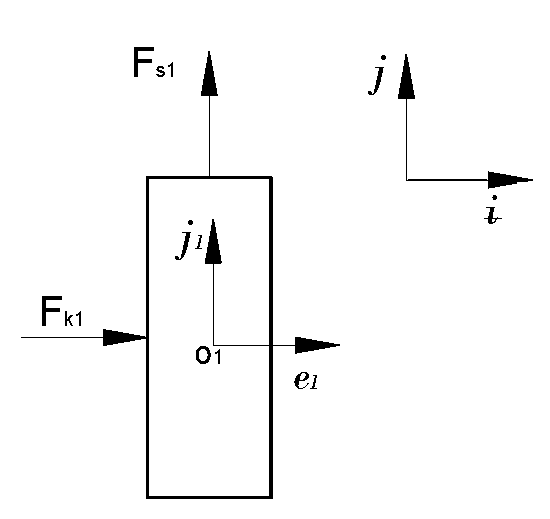
\includegraphics[width=0.8\textwidth]{Chapter4/fig/ForceWheel1}
		\caption{External Force on Rear Wheel}\label{fig:ForceRearWheel}
	\end{minipage}
	\hfill
	\begin{minipage}[t]{0.5\textwidth}
		\centering
		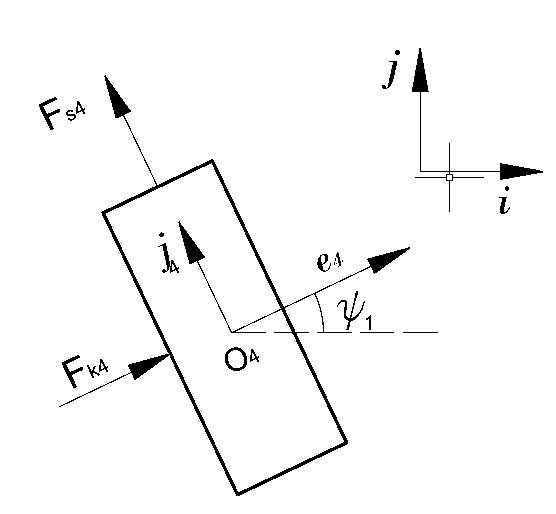
\includegraphics[width=0.8\textwidth]{Chapter4/fig/ForceWheel2}
		\caption{External Forces on Front Wheel }\label{fig:ForceFrontWheel}
	\end{minipage}
	%\caption{Actuator effort}
\end{figure} 
The $T_i$ has all ready been calculated in the above section, the $w_i^w$ term is derived next. Where, $w_i^w$ is the working wrench acting on the individual bodies. This consist of all the external forces such as actuator force, friction force and gravitational force.
The forces acting wheel 1,as shown in Figure \ref{fig:ForceRearWheel},  are the friction force due longitudinal slip $Fs_1$ and frictional force  due to lateral slip or skidding, $Fk_1$ at the ground-wheel interface . The motor torque action on the wheel 1 is $\tau_{m1}$.  Similarly forces acting on wheel 2 are $Fs_2$, $Fk_2$ and $\tau_{m2}$. Therefore, $w_1$ and $w_2$ are written as 
\[ w_n=\begin{pmatrix}
\tau_{m,n}i\\
F_{k,n}i+F_{s,n}j
\end{pmatrix},  \quad n=\{1,2\}\]

The front wheels have steering actuation, let the steering  torques be represented by $\tau_{s,4}$ and  $\tau_{s,4}$. The friction forces on the front steered wheel is shown in \ref{fig:ForceFrontWheel} act along $\{e_4,f_4\}$ and $\{e_5,f_5\}$ for the two front wheels. No traction force is applied to the front wheels. Therefore, $w_4$ and $w_5$ is given by
\[ w_n=\begin{pmatrix}
\tau_{s,n}k\\
F_{k,n}e_n+F_{s,n}f_n
\end{pmatrix},  \quad n=\{4,5\}\]
Since no external force is acting on the platform, i.e. body \#3. \[w_3=0_{6x1}\]

We can now calculate $T_i^Tw_i$

\begin{subequations}
	\label{eqn:slip_Tau_is}
	\begin{align}
	T_1^T w_1&=\begin{pmatrix}
	\tau_{m1} & 0 & F_{s1}& 0& F_{k1}&0&0&0&0
	\end{pmatrix} ^T\\
	T_2^T w_2&=\begin{pmatrix}
	0&\tau_{m2}& 0&F_{s2}&  F_{k2}&0&0&0&0
	\end{pmatrix} ^T\\
	T_3^T w_3&=0_{9x1} \quad \text{since } w_3=0\\
	T_4w_4&= \begin{pmatrix}
	0 & 0& \alpha_1& \alpha_2 & \alpha_3 &\tau_{s4}& 0&0 &0
	\end{pmatrix}^T\\
	T_5w_5&=\begin{pmatrix}
	0 & 0& \beta_1& \beta_2 & \beta_3 &0 &\tau_{s5}& 0&0
	\end{pmatrix}^T
	\end{align}
\end{subequations}
Where 
\[\alpha_1=-\frac{\tau_{s4}}{l}+\lambda_1(F_{k4}C_{\phi_1}-F_{s4}S_{\phi_1})+\lambda_3(F_{k4}S_{\phi_1}+F_{s4}C_{\phi_1})\]
\[\alpha_2=\frac{\tau_{s4}}{l}-\lambda_1(F_{k4}C_{\phi_1}-F_{s4}S_{\phi_1})+\lambda_2(F_{k4}S_{\phi_1}+F_{s4}C_{\phi_1})\]
\[\alpha_3=(F_{k4}C_{\phi_1}-F_{s4}S_{\phi_1})\]
\[\beta_1=-\frac{\tau_{s5}}{l}+\lambda_1(F_{k5}C_{\phi_2}-F_{s5}S_{\phi_2})+\lambda_2(F_{k5}S_{\phi_2}+F_{s5}C_{\phi_2})\]
\[\beta_2=\frac{\tau_{s5}}{l}-\lambda_1(F_{k5}C_{\phi_2}-F_{s5}S_{\phi_2})+\lambda_3(F_{k5}S_{\phi_2}+F_{s5}C_{\phi_2})\]
\[\beta_3=(F_{k5}C_{\phi_2}-F_{s5}S_{\phi_2})\]
Therefore the $\tau$ of Equation \ref{eqn:slipTauSum} can be written as
\begin{equation}
\tau=\begin{pmatrix}
\tau_{m1} & \tau_{m2} & (F_{s1}+\alpha_1+\beta_1)&( F_{s2}+\alpha_2+\beta_2)&  (F_{k1}+ F_{k2}+\alpha_3+\beta_3)& \tau_{s4}&\tau_{s5} &0&0
\end{pmatrix}^T
\end{equation}
\subsection{Simulation}

\section{Dynamical Model of Steering System}
The dynamical model of the steering system shown in Figure \ref{fig:SteerAsm} was derived  using Lagrangian method. The equations of motion were derived under the assumptions,  that the vehicle body \#3 was at rest and second that the mass of links \#8 and \#9 were negligible compared to other links. The kinematic energy of all the body except \#8 and \#9 is presented next.


 


The kinetic energy of link  \#6 is given by
\begin{equation}
 K_6=\frac{1}{2}(m_6((x^b_6)^2+(y^b_6)^2)+I_{6zz})\dot{\phi_6}
\end{equation}
 where, $m_6$ is the mass, $(x^b_6,y^b_6)$  the coordinate of c.m.  expressed  in the body co-ordinate frame $B:\{i_6,j_6,k_6\}$ as shown in Figure \ref{fig:SteerLink} and $I_{6zz}$ is the moment of inertia in the body coordinate of link \#6.
 
 
 Next we derive the kinetic energy of body \# 4, the wheel. 
 The coordinate of c.g of wheel, $O_4$ in the world  $F:\{i,j,k\}$  is given by \[ \begin{pmatrix}
x_{4}\\y_{4} \end{pmatrix}_F
= \begin{pmatrix}-\frac{l}{2} \\0
\end{pmatrix}+
\begin{pmatrix}
		\cos\phi_6 &  -\sin\phi_6\\ -\sin\phi_6 & \cos\phi_6
\end{pmatrix} + 
\begin{pmatrix}
			-l_3\\0
\end{pmatrix}\]
\begin{figure}
	\begin{minipage}[t]{0.5\textwidth}
		\centering
		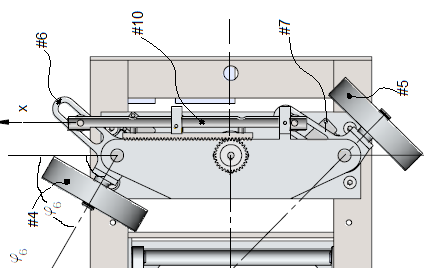
\includegraphics[width=3in]{Chapter4/fig/SteerModel} 
		\caption{Steering Assembly}\label{fig:SteerAsm}
	\end{minipage}
	\hfill
	\begin{minipage}[t]{0.5\textwidth}
		\centering
		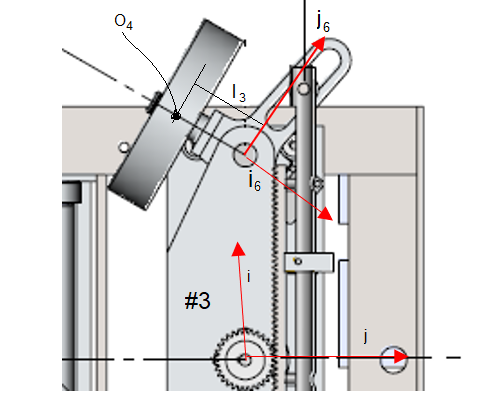
\includegraphics[width=2in]{Chapter4/fig/link} 
		\caption{Link }\label{fig:SteerLink}
	\end{minipage}
	%\caption{Actuator effort}
\end{figure}
 	
  The linear velocity $\dot{O}_4$  and its angular velocity $\omega_6$  expressed in the world frame $F:\{i,j,k\}$ is given by
 \begin{eqnarray}
 \dot{O}_4=l_6\dot{\phi_6}[\sin\phi_6, ~ -\cos\phi_6] ^T
 \end{eqnarray}
 
 \begin{equation}
 \omega_6=\dot\phi_6k_6+\dot\theta_4i_6 ~=~ [\dot\theta_4\cos\phi_6,~ \dot\theta_4\sin\phi_6,~ \dot\phi_6]^T
 \end{equation} where, $l_6$ is the length as shown in Figure \ref{fig:SteerLink}  and $\dot\theta_4$ is the spinning rate of the wheel about axis $i_6$.
 Then the kinetic energy of body \#4 is given by
\begin{equation}
 K_4=\frac{1}{2}(m\dot O_4 ^T ~\dot O_4+ \omega_6^T [I_6]_F~\omega_6  )
 \end{equation}
 \begin{multline}
 K_4=\frac{1}{2} l_6^2 \dot\phi_6 m \begin{pmatrix}
 \sin\phi_6, ~ -\cos\phi_6
 \end{pmatrix}
 \begin{pmatrix}
 \sin\phi_6\\ -\cos\phi_6
 \end{pmatrix}\\
 + 
 \begin{pmatrix}
 \dot\theta_4 \cos\phi_6, ~ \dot\theta_4 \sin\phi_6, ~\dot\phi_6
 \end{pmatrix}[I_6]_F
 \begin{pmatrix}
 \dot\theta_4 \cos\phi_6\\ \dot\theta_4 \sin\phi_6\\ \dot\phi_6
 \end{pmatrix}
 \end{multline} Where $[I_6]_F$ is the inertia matrix of wheel about its c.g. expressed in world frame $F$.
 In general the moment of inertia matrix of the body is known in the body frame $B$, ie $[I_6]_B$. This can be transformed to the world coordinate frame $F$ by using the formula
 \[ [I_4]_F=R^F_B[I_4]_B [R^F_B]^T\] where, $R^F_B$ represents rotation transformation matrix between the fixed Frame, $F$, and the body frame, $B$. 
 The above Equation, after above transformation can be written as
 \begin{equation}
 K_4=\frac{1}{2}(l_3^2\dot\phi_6^2m_4+[I_{4xx}]_B\theta_4^2)
 \end{equation} 
where, $I_{4zz} $ is the moment of inertia of the wheel about its z axis in the body coordinate frame.

The kinetic energy of the tie rod, i.e., body \#10, which under goes linear reciprocating motion in a plane is given by
\begin{equation}
K_{10}=\half m_{10} \dot{x}
\end{equation} where, $x$ is the displacement of the tie rod and $m_{10}$ is its mass.


The kinetic energy of body \#5, i.e., second wheel and second link \#7 can be derived in a similar fashion as that of body \#4 and \#6 respectively. The kinetic energy of body \#7 is given as
\begin{equation}
K_7=\frac{1}{2}(m_7((x^b_7)^2+(y^b_7)^2)+I_{7zz})\dot{\phi_7}
\end{equation}
where, $m_7$ is the mass and  $I_{7xx}$ moment of inertia of body \#7 .

The kinetic energy of body \#5  is given as
 \begin{equation}
K_4=\frac{1}{2}(l_3^2\dot\phi_7^2m_5+[I_{5xx}]_B\theta_5^2)
\end{equation} 
 where $m_5$  is the mass and $I_{5xx}$ moment of inertia of body \#5.
 

From the geometry of Figure \ref{fig:davis} following relations can be derived 
\begin{equation}
\label{eqn:thetaTox}
\tan(\alpha-\phi_6)=\frac{b+x}{h}, \quad \quad \tan(\alpha-\phi_7)=\frac{b-x}{h}
\end{equation}
\begin{equation}
\label{ro}
x^b_6+y^b_6=x^b_7+y^b_7=r_0
\end{equation}
\begin{equation}
\dot{\phi_6}=\dfrac{h\dot x}{h^2+b^2+2bx+x^2}=f_1(x)\dot x,\quad \dot{\phi_7}=\dfrac{h\dot x}{h^2+b^2-2bx+x^2}=f_2(x)\dot x
\end{equation}
 Therefore the total kinetic energy of steering unit is 
\[K_s=\sum_{i=4..10}K_i\]
using the expression for $K_i$  and using Equations 4.48, 4.49 and 4.50, the above equation for $K_s$  is written as 
\begin{multline}
	K_s=\frac{\dot x^2}{2} \left( m_{10}+(m_l r^2_0+I{zz})+l^2_3m_w \right) \left(f^2_1(x)+f^2_2(x) \right)\\ + \half I_{wxx}\left(\dot\theta^2_4  +\dot\theta^2_5\right)
\end{multline}
under the following assumptions \[l_3=l_4, \quad m_4=m_5=m_w, \quad m_6=m_7=m_l, \quad I_{7zz}=I_{6zz}=I_{zz}\]
The Lagrangian in this case is simply the kinetic energy, i.e,  $L=K_s$. Since the external forces acts only along the $x$ ordinate, via steering motor. We get
\[F_x= \dfrac{\partial}{\partial t}\dfrac{\partial L}{\partial \dot x} - \dfrac{\partial L}{\partial x}\]
or 
\begin{multline}
\label{eqn:SteerDyn}
F_x=\ddot{x}\left[ m_{10}+\left(m_lr_o^2+I{zz}+l^2_3m_w \right) \right] \left( f_1^2+f_2^2 \right)\\
+2\dot x^2 \left(m_lr^2+I{zz}+l_3^2 m_w \right) \left( f_1 \dot f_1 +f_2 \dot f_2\right)+F_1+F_2
\end{multline}
The external force $F_1$ and $F_2$ in the above equation is given by
\[F_i=\dfrac{T_s}{h},i={1,2} \]
where $T_s$ is evaluated using Equation \ref{eqn:brake} assuming symmetric loading of both the wheels. The derivative of $f_1(x)$ and  $f_2(x)$ is given by 
\[ \dfrac{df_1}{dt}=-\dfrac{2(x+b)h}{(h^2+b^2+2bx+x^2)^2}, \quad \dfrac{df_2}{dt}=-\dfrac{2(x-b)h}{(h^2+b^2-2bx+x^2)^2}\]



\subsection{Design of PID controller}
To control the steer angle of the front wheels a computed torque controller \cite{craig2005introduction} was designed. If $U$ denotes the auxiliary control input then $F_x$ is given by
\begin{multline}
\label{eqn:SteerCont}
F_x=U\left[ m_{10}+\left(mr_o^2+I{zz}+l^2_3m_w \right) \right] \left( f_1^2+f_2^2 \right)\\
+2\dot x^2 \left(mr^2+I{zz}+l_3^2 m_w \right) \left( f_1 \dot f_1 +f_2 \dot f_2\right) 
+F_1+F_2
\end{multline}
eliminating  $F_x$ using Equation \ref{eqn:SteerDyn} and Equation\ref{eqn:SteerCont}, we get
\begin{equation}
\label{eqn:SteerCont2}
\ddot x =U
\end{equation}
If $x_d$, is the set point for the displacement of the rack of the steering system and $e(t)=(x(t)-x_d)$ is the position error, we define auxiliary input $U$ as  
\begin{equation}
\label{eqn:SteerCont3}
 U=-K_d \dot x -K_p \left(x(t)-x_d \right) -K_i\int e(t)dt \end{equation}
then Equation \ref{eqn:SteerCont2} which represents the overall dynamics of the steering mechanism along with the controller, can  be written as 
\[\ddot e(t) +K_d \dot{e}(t) +K_p e(t)+ K_i\int e(t)dt=0 \]
It is be noted that $\dot e(t)=\dot x$ and $\ddot e(t)=\ddot x$, since $x_d=const$. Given that  $y_1(t)= \int e(t)$ and $Y=[y_1,~y_2,~y_3]^T$, the above equation can be rewritten in state space \[\dot{Y}=AY\] or
\begin{equation}
\begin{pmatrix}
\dot y_1 \\ \dot y_2 \\\dot y_3
\end{pmatrix}
=
\begin{pmatrix}
0 & 1 & 0\\ 0 & 0 & 1\\ -K_i & -K_d & -K_p
\end{pmatrix}
\begin{pmatrix}
 y_1 \\ y_2 \\ y_3
\end{pmatrix}
\end{equation}
With $K_d=20,~K_p=60,~K_i=100 $ the system is stable as  the state transition matrix $A$ has all its eigen values, $\lambda$, with negative real part, as given below 
\[ \lambda= \{-16.7794 + 0.0000i, ~ -1.6103 + 1.8348i, ~ -1..6103 - 1.8348i\}\]
 \textbf{\textit{These controller parameters were arrived by trial and error using multiple simulation. The guiding principle behind the selection of these parameters was to choose one root far away form the imaginary axis so that its dynamics dies very fast with the respect to  the other two roots.  The system then behaves as second order system. The remaining two roots thus governs the dynamics of the system.  they were chosen as complex conjugate with negative real part and near to imaginary axis so as to make the steering unit dynamics  under damped.}}

\subsection{Simulation and results}
The simulation of the  dynamic Equation \ref{eqn:SteerDyn} and controller given by Equations \ref{eqn:SteerCont} and \ref{eqn:SteerCont3} was carried out with the step change in steering angle responding to $ 20~mm$  rack displacemet $(x)$.  The parameter used for the nominal plant were obtained form solid model of the parts and are listed in table \ref{tb:steerPara}. The results of the wheel orientations and the actuator effort required are given in Figure \ref{fig:SteerPos} and \ref{fig:SteerEfort} respectively.

\begin{table}[!htbp]
	\caption{Key parameters steering assembly.}
	\label{tb:steerPara}
	\centering
	\begin{tabular}{l l l }
		\hline
		
		%\emph{Parameter}  & \emph{Example} & \emph{Font size and style} \\
		%\hline
		Wheel Mass& $m_w $ &$ 350~g$  \\ 
		Wheel Inertia & $I_{wxx}$ & $463~ Kg ~mm^2$\\
		Connecting Rod Mass & $m_{10} $& $200~g$ \\
		Link mass& $m_l$ & 80g\\
		Link Inertia & $I_{zz} $& $60834~Kg ~mm^2$\\
		Link Cg distance & $r_o$ & $18mm$\\
		\hline
	\end{tabular}
\end{table}

 
\begin{figure}
	\begin{minipage}[t]{0.5\textwidth}
		\centering
		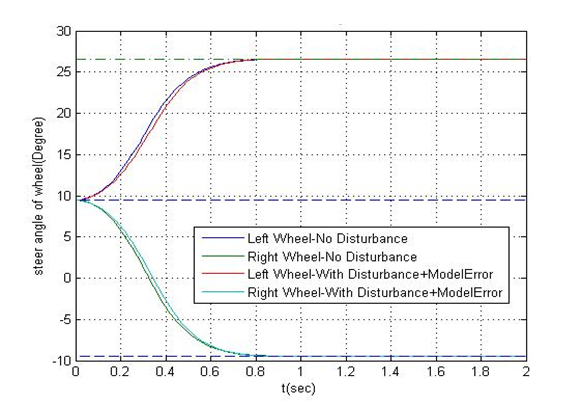
\includegraphics[width=3in]{Chapter4/fig/SteeringPos} 
		\caption{Change in steer angle}\label{fig:SteerPos}
	\end{minipage}
	\hfill
	\begin{minipage}[t]{0.5\textwidth}
		\centering
		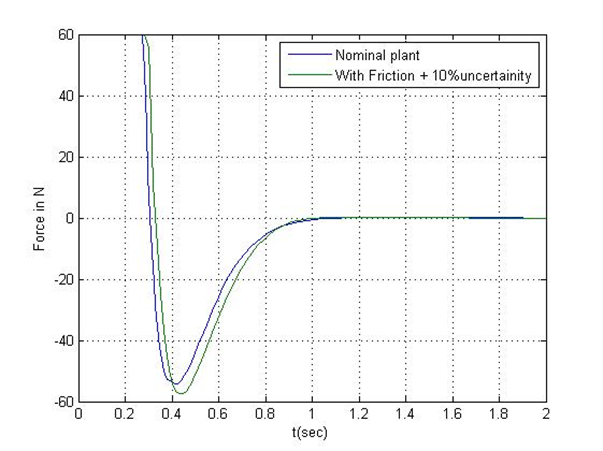
\includegraphics[width=3in]{Chapter4/fig/SteerEffort} 
		\caption{Control effort}\label{fig:SteerEfort}
	\end{minipage}
	%\caption{Actuator effort}
\end{figure} 
The simulation results establishes that with $10\%$ error in plant parameters there is practically no deviation in the performance of the controller. The results also predicts a settling time of $0.8~sec$ for the system. It may be noted that the roll velocity of the wheel does not affect the dynamics of the steering system as is indicated by the absence of $\dot\theta_4$ and $\dot\theta_5$  from Equation \ref{eqn:SteerDyn} .
\section{Summary}
In this chapter, the dynamic equations were derived for  the most general form of passive wheel configuration. Even though  only two passive wheel configuration was considered the same formulation can be extended to any number of  wheels. It is shown that the  dynamics of standard caster wheels is a special case of the  general case with $d_1=0$. It is also proven why a caster needs  non-zero caster offset. There is a  need of extra actuator in case $d_2=0$. The dynamic equation for the Davis steering mechanism was formulated and using  simulation the settling time for the same was obtained.
    




